
\section{Terceira Questão (9 pts)}

\subsection{Análise Analítica}

\numberwithin{equation}{section}
\numberwithin{figure}{section}

Para modelar o problema dado, temos que partir das equações de Navier-Stokes e 
da equação de conservação da massa. Assumindo escoamento incompressível (massa específica constante),
temos

\begin{equation}\label{eq:Q3NS1}
    \begin{split}
        \rho\left(\diffp{u}{t} + u\diffp{u}{x} + v\diffp{u}{y}+ w\diffp{u}{z}\right) \\
         = \rho g_x - \diffp{p}{x} + \mu \left(\diffp[2]{u}{x} + \diffp[2]{u}{y} + \diffp[2]{u}{z}\right)
    \end{split}
\end{equation}

\begin{equation}\label{eq:Q3NS2}
    \begin{split}
        \rho\left(\diffp{v}{t} + u\diffp{v}{x} + v\diffp{v}{y}+ w\diffp{v}{z}\right) \\
         = \rho g_y - \diffp{p}{y} + \mu \left(\diffp[2]{v}{x} + \diffp[2]{v}{y} + \diffp[2]{v}{z}\right)
    \end{split}
\end{equation}

\begin{equation}\label{eq:Q3NS3}
    \begin{split}
        \rho\left(\diffp{w}{t} + u\diffp{w}{x} + v\diffp{w}{y}+ w\diffp{w}{z}\right) \\
         = \rho g_z - \diffp{p}{z} + \mu \left(\diffp[2]{w}{x} + \diffp[2]{w}{y} + \diffp[2]{w}{z}\right)
    \end{split}
\end{equation}

\begin{equation}\label{eq:MassConservation}
    \nabla \cdot V = 0 \logo \diffp{u}{x} + \diffp{v}{y} + \diffp{w}{z} = 0
\end{equation}

As equações \eqref{eq:Q3NS1}, \eqref{eq:Q3NS2} e \eqref{eq:Q3NS3} são as três 
equações de Navier-Stokes, e a equação \eqref{eq:MassConservation} é a equação de conservação
da massa.

Com base nos dados do problema, podemos fazer várias simplificações nas equações acima:

\begin{itemize}
    \item Escoamento unidimensional apenas na direção $x$: $v = w = 0$
    \item Escoamento em regime permanente: $\diffp{u}{t} = 0$
    \item Gravidade atua apenas na componente $y$: $g_x = g_z = 0$
    \item Escoamento plenamente desenvolvido: $\diffp{u}{x} = \diffp[2]{u}{x} = 0$
    \item Na geometria analisada, o sistema de coordenadas possui apenas eixos $x$ e $y$: 
    $\diffp{u}{z} = \diffp[2]{u}{z} = 0$ 
\end{itemize}

Com todas essas simplificações, as equações acima se reduzem a 

\begin{equation}\label{eq:q3modelo}
    \mu\diffp[2]{u}{y} - \diff{p}{x} = 0
\end{equation}

\noindent em que $u$ é função de apenas uma variável $y$.
Assim, temos as seguintes condições de contorno para \eqref{eq:q3modelo}:

\begin{equation}\label{eq:q3modeloContorno}
    \begin{cases}
        u(-h) = 0, \\
        u(h) = U
    \end{cases}
\end{equation}

A Figura \ref*{fig:geometriaQ3} exibe a geometria do Problema 3, para melhor visualizar as 
condições de contorno e o sistema de coordenadas adotado. Veja que, novamente por simetria,
precisamos analisar apenas o que acontece em uma linha vertical da placa inferior até a placa
superior para modelar o escoamento inteiro.

\begin{figure}[h!]
    \caption{Geometria da questão 3.}
    \label{fig:geometriaQ3}
    \centering
    \centerline{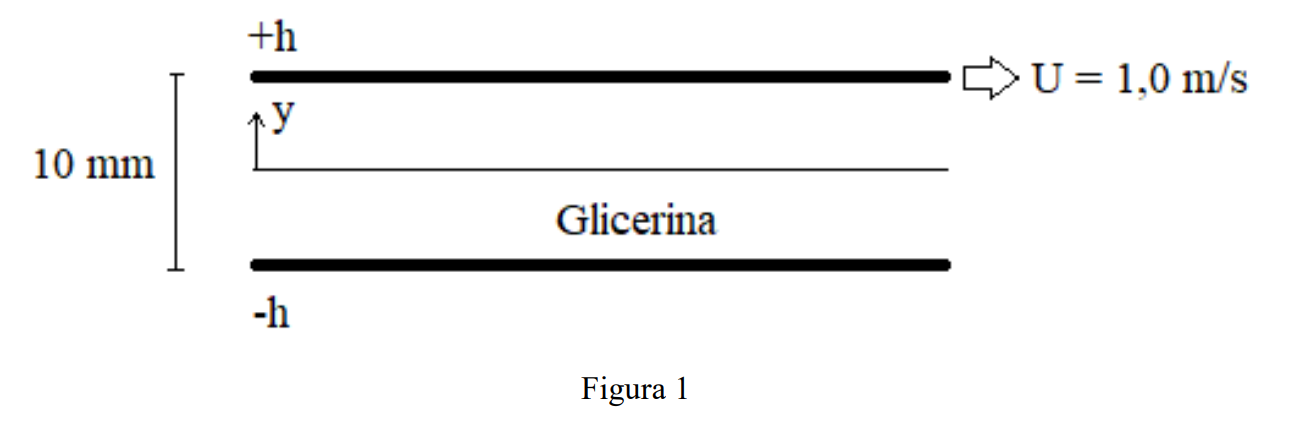
\includegraphics[scale=0.3]{geometriaQ3.png}}
    \par{Fonte: Huebner, R. (2023).}
\end{figure}

De modo semelhante ao feito na Questão 2, podemos tentar obter uma solução analítica
para o modelo através de integração direta, assumindo que o gradiente de pressão 
na direção do escoamento $\diff{p}{x}$ é constante.

\[ \diffp[2]{u}{y} = \diff{p}{x} \frac{1}{\mu} \]

\[ \int \diffp{u}{y} \, dy = \int y\diff{p}{x}\frac{1}{\mu} + C_1  \, dy \]

\begin{equation}\label{eq:q3solucaoGeral}
    u(y) = \frac{y^2}{2}\diff{p}{x}\frac{1}{\mu} + yC_1 + C_2 
\end{equation}

\eqref{eq:q3solucaoGeral} é a solução geral da EDP \eqref{eq:q3modelo}. Com as condições de contorno,
temos

\[
    \begin{cases}
        0 = \frac{(-h)^2}{2}\diff{p}{x}\frac{1}{\mu} - hC_1 + C_2 , \\
        U = \frac{h^2}{2}\diff{p}{x}\frac{1}{\mu} + hC_1 + C_2 
    \end{cases} 
\]  

\noindent somando as duas equações, temos  

\[ U = h^2\diff{p}{x}\frac{1}{\mu} + 2C_2 \]

\[ C_2 = \frac{1}{2} \left(U - h^2\diff{p}{x}\frac{1}{\mu}\right)  \]

Agora substituimos esse $C_2$ calculado de volta, para achar o $C_1$:

\[ 0 = \frac{h^2}{2}\diff{p}{x}\frac{1}{\mu} - hC_1 + \frac{1}{2} \left(U - h^2\diff{p}{x}\frac{1}{\mu}\right)  \]

\[ 0 = \frac{h^2}{2}\diff{p}{x}\frac{1}{\mu} - hC_1 + \frac{1}{2}U - \frac{1}{2} h^2\diff{p}{x}\frac{1}{\mu} \]

\[ - \frac{1}{2}U = - hC_1 \logo C_1 = \frac{U}{2h} \]

Finalmente, a solução analítica de \eqref{eq:q3modelo} com as condições de contorno de 
\eqref{eq:q3modeloContorno} é

\[ u(y) = \frac{y^2}{2}\diff{p}{x}\frac{1}{\mu} + y\frac{U}{2h} + \frac{1}{2} \left(U - h^2\diff{p}{x}\frac{1}{\mu}\right)  \]

\[ u(y) = \frac{y^2}{2}\diff{p}{x}\frac{1}{\mu} + y\frac{U}{2h} + \frac{1}{2}U - \frac{1}{2} h^2\diff{p}{x}\frac{1}{\mu}  \]

\[ \frac{u(y)}{U} = \frac{y^2}{2U}\diff{p}{x}\frac{1}{\mu} + \frac{y}{2h} + \frac{1}{2} - \frac{1}{2U} h^2\diff{p}{x}\frac{1}{\mu}  \]

\[ \frac{u(y)}{U} = \frac{1}{2} \left(1 + \frac{y}{h}\right) -  \diff{p}{x} \frac{h^2}{2\mu U} \left(1 -  \frac{y^2}{h^2} \right) \]

\noindent definimos $P$ tal que

\[ P = - \diff{p}{x}  \frac{h^2}{2\mu U} \]

\noindent e assim podemos reescrever a expressão como

\begin{equation}\label{eq:solucaoAnalitica}
    \frac{u(y)}{U} = \frac{1}{2} \left(1 + \frac{y}{h}\right) + P\left(1 - \frac{y^2}{h^2}\right) 
\end{equation}

Usamos os seguintes parâmetros:

\begin{itemize}
    \item Domínio de análise vertical: $-h \leq y \leq h$, com $h = 5 \un{mm}$
    \item Viscosidade: $\mu=1.49 \un{ kg m$^{-1}$ s$^{-1}$}$
    \item Velocidade de deslocamento da placa superior: $U=1 \un{m/s}$
    \item Gradiente de pressão: $\diff{p}{x} = -178800 \un{Pa}$
\end{itemize}

Com \eqref{eq:solucaoAnalitica} e os parâmetros, podemos obter a distribuição de velocidades
do fluido analiticamete. A Figura \eqref{fig:graficoAnaliticoQ3} exibe a solução obtida.

\begin{figure}[h!]
    \caption{Solução analítica da questão 3.}
    \label{fig:graficoAnaliticoQ3}
    \centering
    \centerline{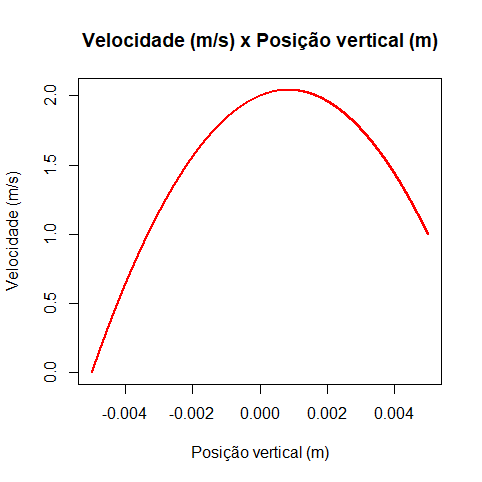
\includegraphics[scale=0.7]{graficoAnaliticoQ3.png}}
    \par{Fonte: elaboração própria.}
\end{figure}

Na Figura \eqref{fig:graficoAnaliticoQ3} temos um perfil parabólico para um escoamento plenamente
desenvolvido, conforme visto nas aulas da disciplina. Note que a velocidade máxima está quase no centro,
deslocada devido ao movimento da placa superior.

\subsection{Análise Numérica}

Vamos discretizar \eqref{eq:q3modelo} com o método das difenças finitas. Note que
usamos o diferencial de pressão como constante, logo ele não precisa ser discretizado.
Além disso, como o regime é permanente, usamos o método implícito.

\[ \frac{u_{i+1} - 2u_i + u_{i-1}}{\left(\Delta y\right)^2} = \diff{p}{x} \frac{1}{\mu} \]

\begin{equation}\label{eq:q3Discretizada}
    u_{i+1} - 2u_i + u_{i-1} = \left(\Delta y\right)^2\diff{p}{x} \frac{1}{\mu}
\end{equation}

A equação \eqref{eq:q3Discretizada} é a equação para todos os nós internos no domínio. Nos contornos,
de modo bem parecido como feito no Problema 2, temos, para $i = -h$,

\begin{equation}\label{eq:q3DiscContorno0}
    u_i = 0
\end{equation}

\noindent que corresponde ao ponto de contato do fluido com a placa inferior, em repouso.
Similarmente, quando $i = h$, temos 

\begin{equation}\label{eq:q3DiscContornoU}
    u_i = U
\end{equation}

\noindent que corresponde ao ponto de contato do fluido com a placa superior, com velocidade
igual a $U$.

O algoritmo usado na solução é precisamente o mesmo da questão 2, apenas trocando as equações e os parâmetros físicos.
Continuamos percorrendo cada $\Delta y$, identificando se ele é um nó interno, borda inferior ou
de borda superior, e salvando os coeficientes nas matrizes. No final, resolvemos o sistema linear 
e obtemos o vetor solução.

O código completo feito em R nessa questão está disponível no ANEXO C. Repare que sua estrutura
é a mesma que o código no ANEXO B. A Figura \ref*{fig:graficoNumericoQ3} exibe uma comparação entre
as curvas obtidas analiticamente e numericamente para vários valores de $N$, onde $N = 2h / \Delta y$.

\begin{figure*}[h!]
    \caption{Solução numérica (azul) e solução analítica (vermelha) para vários valores de $N$.}
    \label{fig:graficoNumericoQ3}
    \centering
    \centerline{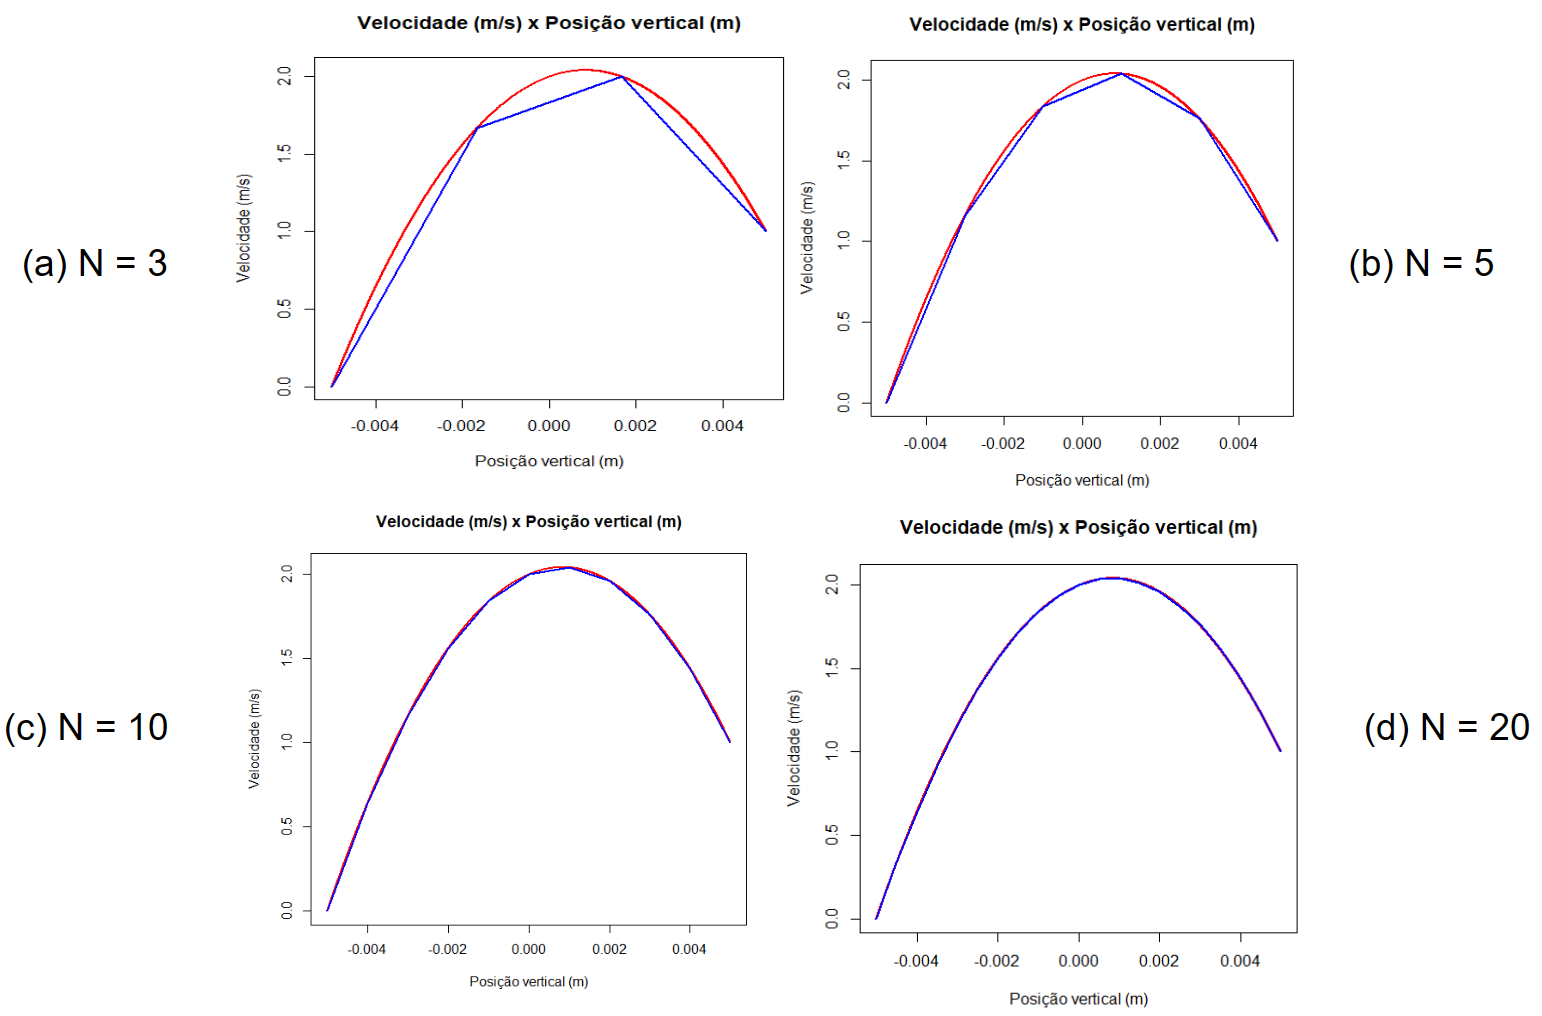
\includegraphics[scale=0.5]{graficoNumericoQ3.png}}
    \par{Fonte: elaboração própria.}
\end{figure*}

De modo bastante semelhante ao visto no Problema 2, na Figura \ref*{fig:graficoNumericoQ3} (a) vemos que
o baixo de valor $N$ resulta em um modelo de pouca exatidão, com o baixo número de pontos discretizados tornando
as aproximações lineares insuficientes para modelar a solução analítica, que é quadrática.

Conforme o valor de $N$ aumenta, temos que as aproximações ficam cada vez melhores, e a partir $N \geq 10$ o modelo
numérico já está bastante parecido com a solução analítica, como mostram as Figuras \ref*{fig:graficoNumericoQ3} (c) e (d).